
\chapter{DynELA plasticity sample cases}

\startcontents[chapters]
\printmyminitoc[1]\LETTRINE{T}his chapter deals with some numerical applications of
the \Dynela~for plasticity applications in 2D, axi-symmetric and
3D cases. In the subsequent tests, if not specified, a Johnson-Cook
constitutive law is used to model the behavior of the material. The
Johnson-Cook hardening flow law is probably the most widely used flow
law for the simulation of high strain rate deformation processes taking
into account plastic strain, plastic strain rate and temperature effects.
Since a lot of efforts have been made in the past to identify the
constitutive flow law parameters for many materials, it is implemented
in numerous Finite Element codes such as Abaqus \cite{abaqus20146}.
The general formulation of the Johnson-Cook law $\sigma^{y}(\overline{\varepsilon}^{p},\stackrel{\bullet}{\overline{\varepsilon}^{p}},T)$
is given by the following equation:

\begin{equation}
\sigma^{y}=\left(A+B\overline{\varepsilon}^{p^{n}}\right)\left[1+C\ln\left(\frac{\stackrel{\bullet}{\overline{\varepsilon}^{p}}}{\stackrel{\bullet}{\overline{\varepsilon}_{0}}}\right)\right]\left[1-\left(\frac{T-T_{0}}{T_{m}-T_{0}}\right)^{m}\right]\label{eq:Samples!Johnson-Cook}
\end{equation}
where $\stackrel{\bullet}{\overline{\varepsilon}_{0}}$ is the reference
strain rate, $T_{0}$ and $T_{m}$ are the reference temperature and
the melting temperature of the material respectively and $A$, $B$,
$C$, $n$ and $m$ are the five constitutive flow law parameters.
A 42CrMo4 steel following the Johnson-Cook behavior law has been selected
for all those tests, and material properties are reported in Table
\ref{tab:Samples!JohnsonCookParameters}.

\begin{table}[h]
\begin{center}\begin{tcolorbox}[width=.75\textwidth,myTab,tabularx={C|C|C|C|C|C|C}]
$E$ & $\nu$ & $A$ & $B$ & $C$ & $n$ & $m$ \\
\small{($Gpa$)} &  & \small{($MPa$)} & \small{($MPa$)} &  &  & \\ \hline
$206.9$ & $0.3$ & $806$ & $614$ & $0.0089$ & $0.168$ & $1.1$ \\ \hline\hline
$\rho$ & $\lambda$ & $C_{p}$ & $\eta$ & $\stackrel{\bullet}{\overline{\varepsilon}_{0}}$ & $T_{0}$ & $T_{m}$ \\
\small{$(kg/m^{3})$} & \small{$(W/m^{\circ}C)$} & \small{$(J/Kg^{\circ}C)$} & & \small{$(s^{-1})$} & \small{$(^{\circ}C)$} & \small{$(^{\circ}C)$} \\ \hline
$7830$ & $34.0$ & $460$ & $0.9$ & $1.0$ & $20$ & $1540$
\end{tcolorbox}\end{center}\caption{Material parameters of the Johnson-Cook behavior for the numerical
tests\label{tab:Samples!JohnsonCookParameters}}
\end{table}


\section{Necking of a circular bar}

\subsection{Axisymmetric Bar Necking}

The necking of a circular bar test is useful to evaluate the performance
of VUMAT subroutine for materials in presence of plasticity and large
deformation \cite{Ponthot2002,SIMO_1998}. Because of the symmetric
structure, an axisymmetric quarter model of the specimen is established.
Dimensions of the specimen are reported in Figure \ref{fig:Samples!Plasticity!NeckingAxi}.
The loading is realized through an imposed total displacement of $7\,mm$
along the $\overrightarrow{z}$ axis on the left side of the specimen
while the radial displacement of the same edge is supposed to remain
zero. On the opposite side the axial displacement is restrained while
the radial displacement is free. The mesh consists of $400$ CAX4RT
elements with a refined zone of $200$ elements on the right side
on $1/3$ of the total height. Again, the total simulation time is
set to $t=0.01\,s$ because of the explicit integration scheme adopted. 

\begin{figure}[h]
\begin{centering}
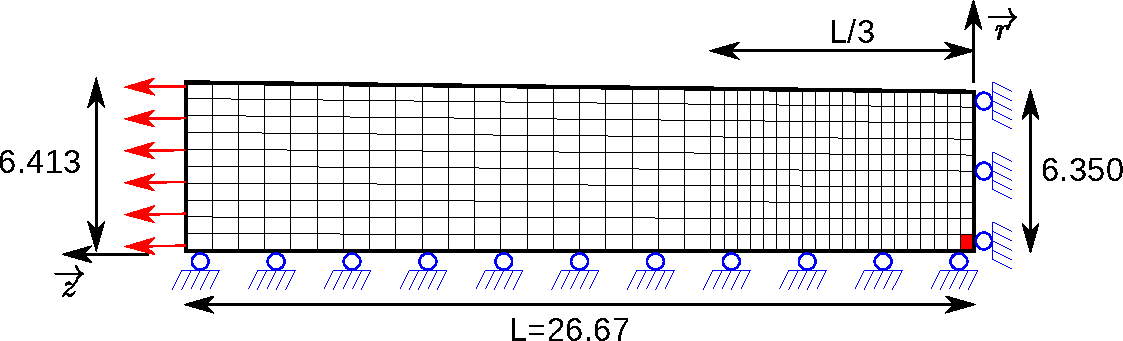
\includegraphics[width=0.75\columnwidth]{Figures/BarNecking}
\par\end{centering}
\caption{Numerical model for the necking of a circular bar\label{fig:Samples!Plasticity!NeckingAxi}}
\end{figure}

Figures \ref{fig:Samples!Plasticity!BarAxi-temp-contour} and \ref{fig:Samples!Plasticity!BarAxi-mises-contour}
shows the temperature $T$ and the von Mises stress $\overline{\sigma}$
contourplots of the deformed rod for both the \Dynela~and Abaqus.
The distributions of the temperatures and stresses are almost the
same for both models. The maximum temperature $T$ is located into
the center element of the model (the red element in Figure \ref{fig:Samples!Plasticity!NeckingAxi})
and the models give quite the same results as reported in Table \ref{tab:Samples!Plasticity!BarAxi-comparison}
for $\overline{\varepsilon}^{p}$, $T$ and the final dimensions of
the specimen $D_{f}$ (final diameter of the necking zone). 

Figure \ref{fig:Samples!Plasticity!BarAxi-comparison} shows the evolution
of the the final dimensions of the specimen $L_{f}$ (final length)
and $R_{f}$ (final radius of the impacting face), the equivalent
plastic strain $\overline{\varepsilon}^{p}$, the temperature $T$,
the von Mises stress $\overline{\sigma}$ and the timeStep $\Delta t$
for the different models for the element at the center of the impacting
face (the red element in Figure \ref{fig:Samples!Plasticity!NeckingAxi}). 

As reported in this figure and according to the results presented
in Table \ref{tab:Samples!Plasticity!BarAxi-comparison}, a quite
good agreement between the results is obtained.

\begin{figure}[h]
\begin{centering}
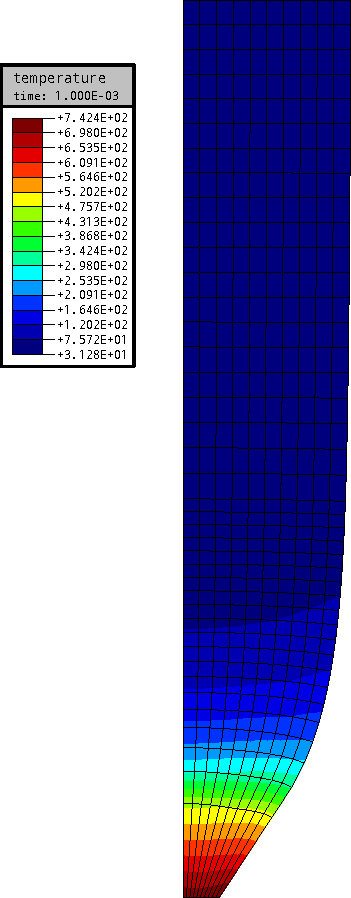
\includegraphics[height=0.5\columnwidth]{Figures/Samples/Plasticity/BarNecking_temperatureCP}\hspace*{3cm}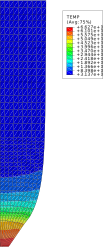
\includegraphics[height=0.5\columnwidth]{Figures/Samples/Plasticity/BarNecking-Abaqus_temperature}
\par\end{centering}
\caption{Temperature $T$ contourplot for the necking of a circular bar (DynELA
left and Abaqus right)\label{fig:Samples!Plasticity!BarAxi-temp-contour}}
\end{figure}

\begin{figure}[h]
\begin{centering}
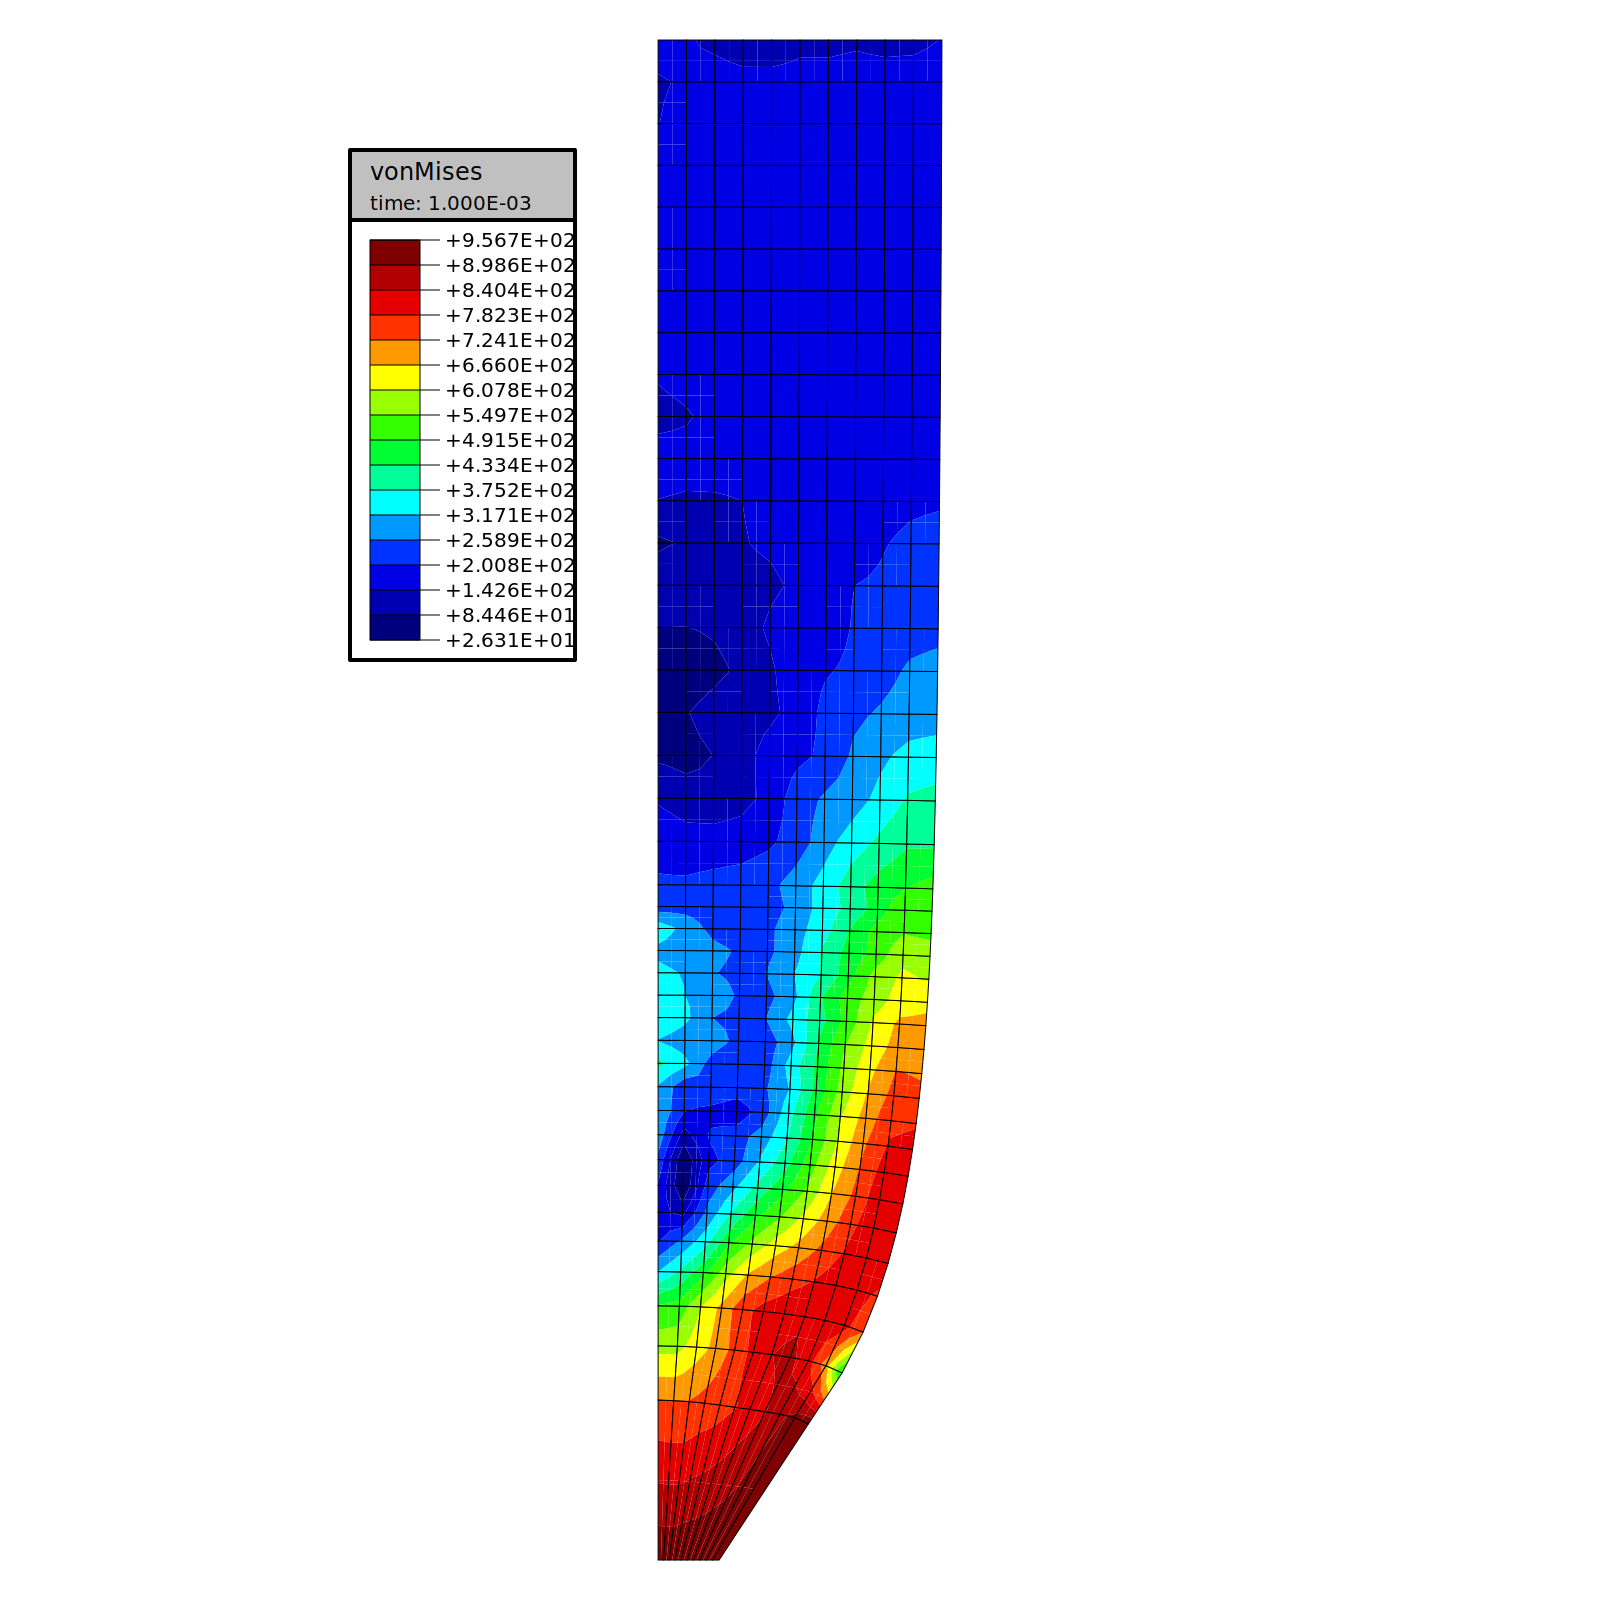
\includegraphics[height=0.5\columnwidth]{Figures/Samples/Plasticity/BarNecking_vonMisesCP}\hspace*{3cm}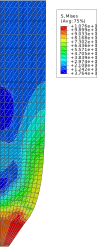
\includegraphics[height=0.5\columnwidth]{Figures/Samples/Plasticity/BarNecking-Abaqus_vonMises}
\par\end{centering}
\caption{von Mises stress $\overline{\sigma}$ contourplot for the necking
of a circular bar (DynELA left and Abaqus right)\label{fig:Samples!Plasticity!BarAxi-mises-contour}}
\end{figure}

\begin{table}[h]
\begin{center}\begin{tcolorbox}[width=.75\textwidth,myTab,tabularx={C|C|C|C}]
code & $D_f$ & $T$ & $\overline{\varepsilon}^{p}$ \\
 & \small{($mm$)} & \small{($^{\circ}C$)} & \\ \hline\hline
DynELA & $2.71$ & $642.78$ & $2.07$ \\ \hline
Abaqus & $2.35$ & $658.91$ & $2.12$
\end{tcolorbox}\end{center}\caption{Comparison of numerical results for the necking of a circular bar
test\label{tab:Samples!Plasticity!BarAxi-comparison}}
\end{table}

\begin{figure}[h]
\begin{centering}
\begin{tabular}{cc}
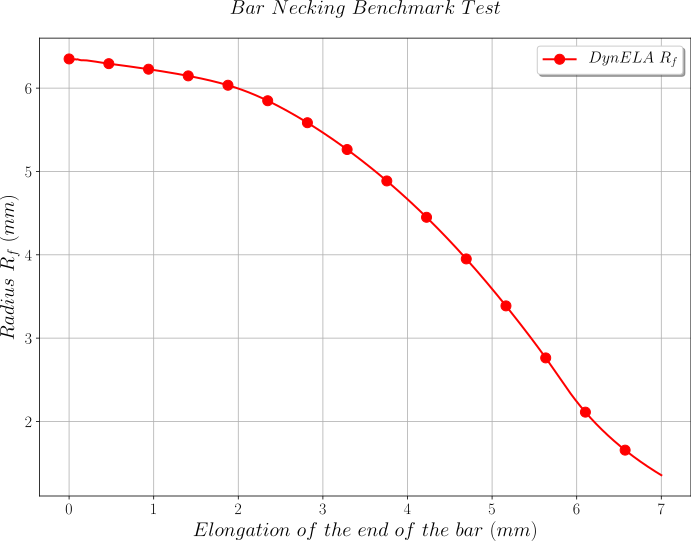
\includegraphics[width=0.45\columnwidth]{Figures/Samples/Plasticity/BarNecking_radius} & 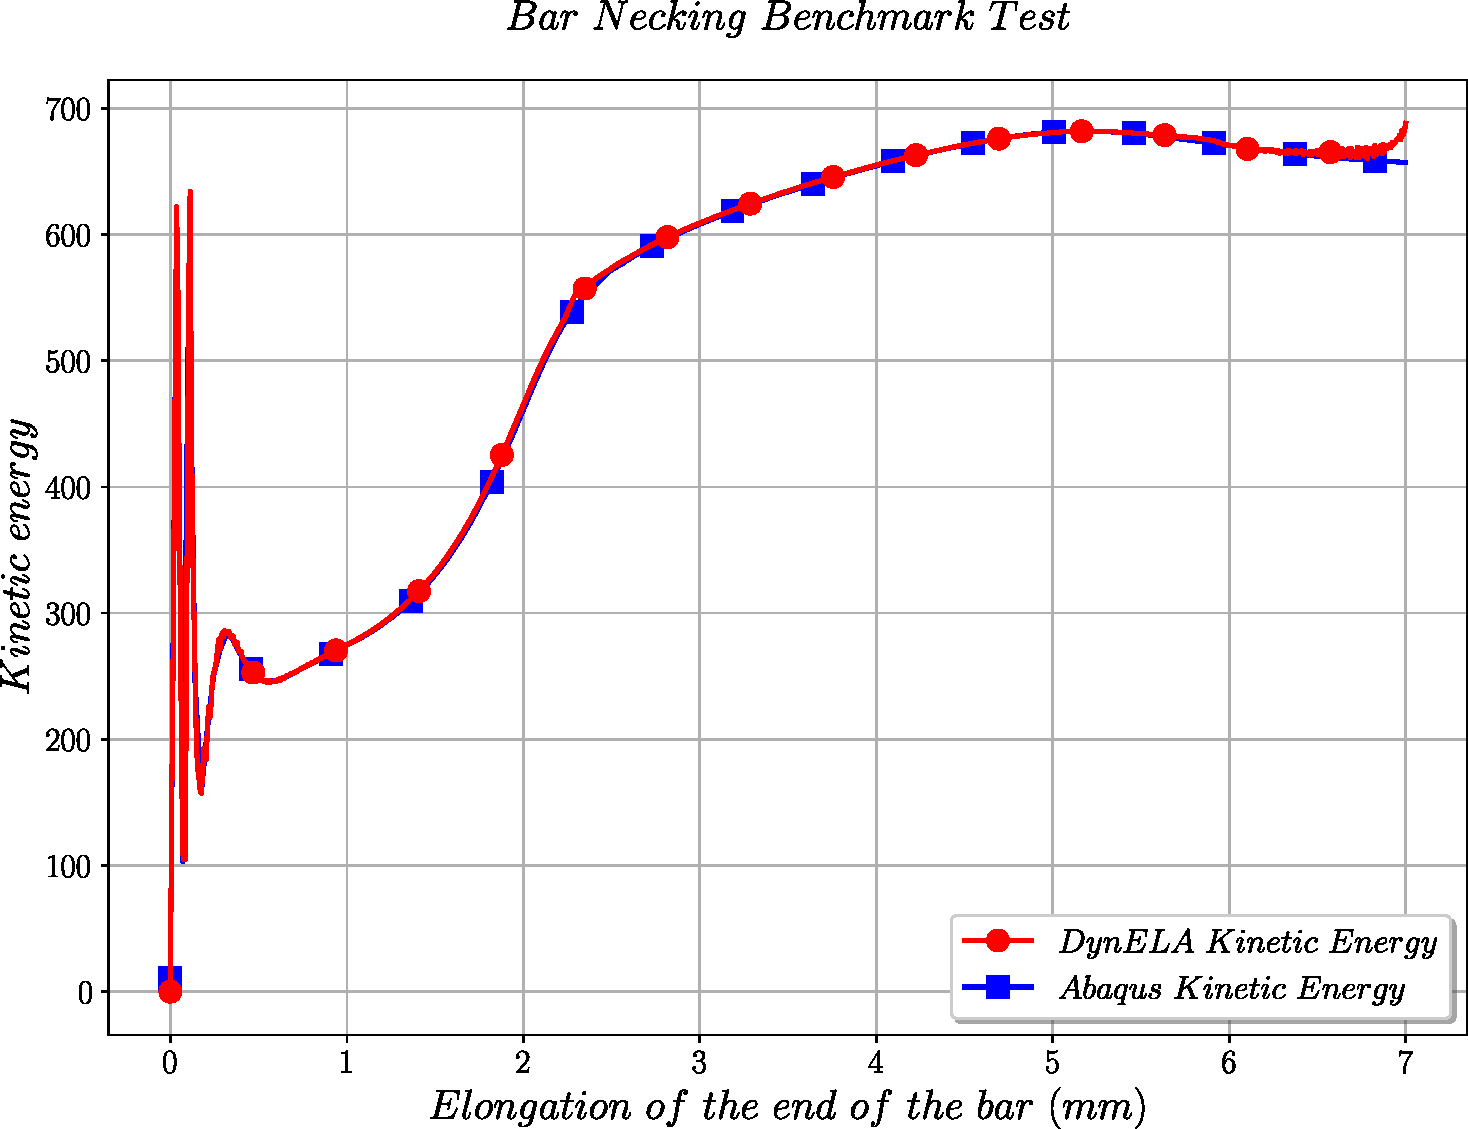
\includegraphics[width=0.45\columnwidth]{Figures/Samples/Plasticity/BarNecking_kineticEnergy}\tabularnewline
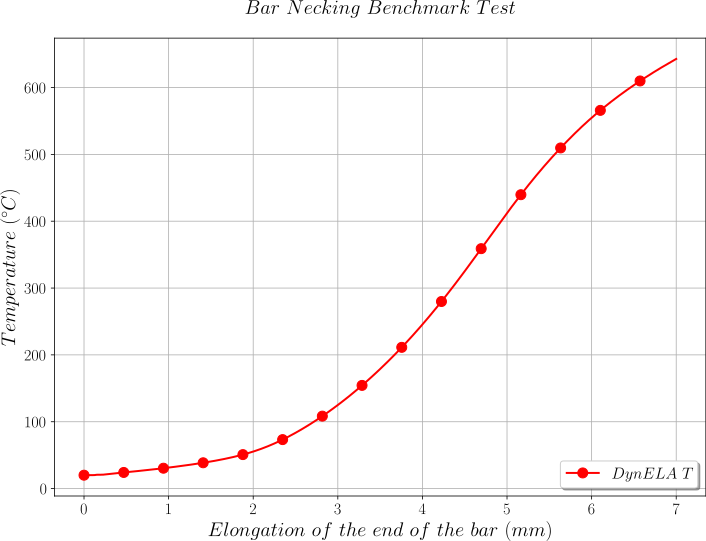
\includegraphics[width=0.45\columnwidth]{Figures/Samples/Plasticity/BarNecking_temperature} & 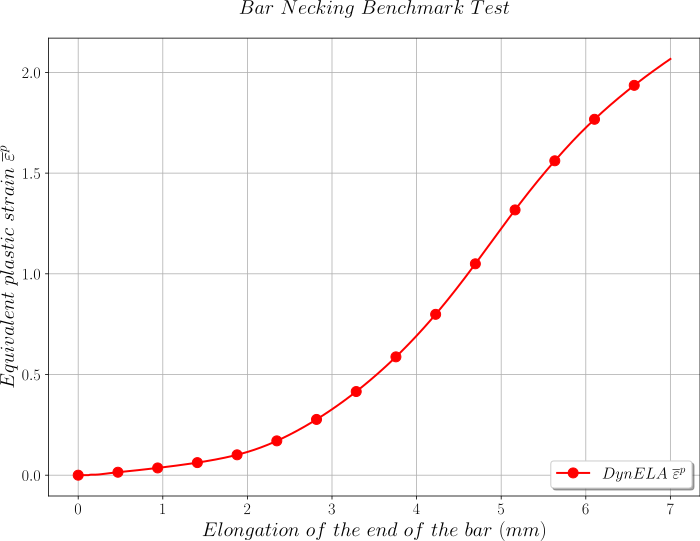
\includegraphics[width=0.45\columnwidth]{Figures/Samples/Plasticity/BarNecking_plasticStrain}\tabularnewline
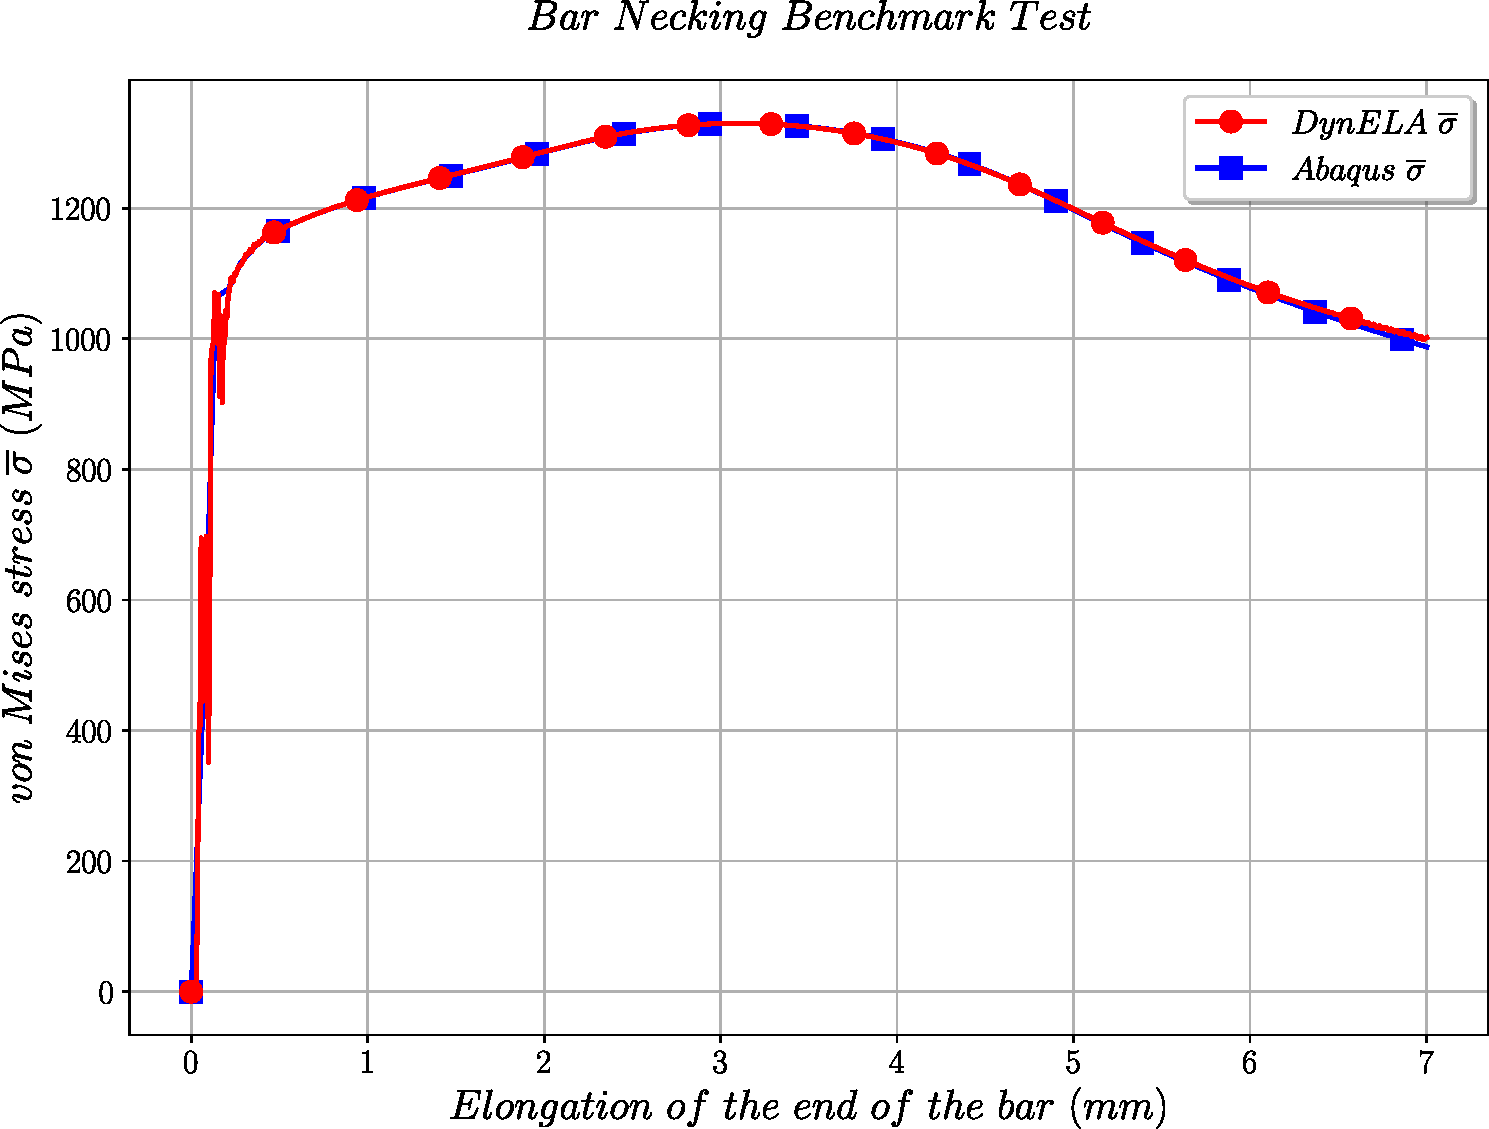
\includegraphics[width=0.45\columnwidth]{Figures/Samples/Plasticity/BarNecking_vonMises} & 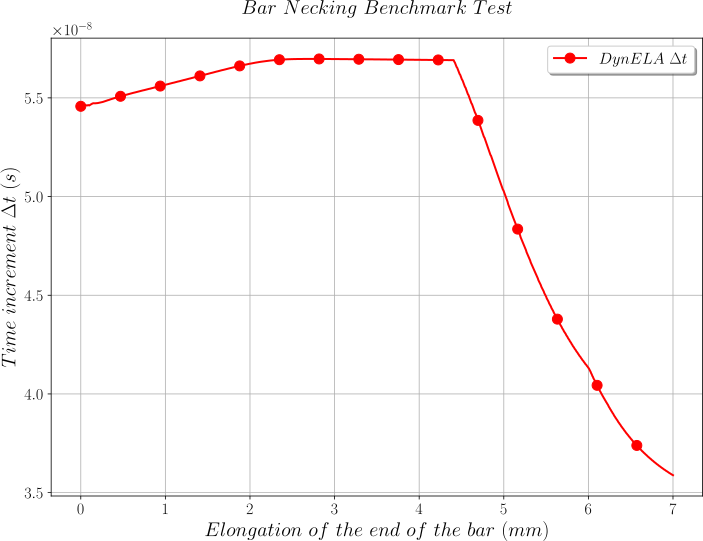
\includegraphics[width=0.45\columnwidth]{Figures/Samples/Plasticity/BarNecking_timeStep}\tabularnewline
\end{tabular}
\par\end{centering}
\caption{Comparison of numerical and analytical results necking of a circular
bar test\label{fig:Samples!Plasticity!BarAxi-comparison}}
\end{figure}

